\begin{figure}
  \centering
  \tikzstyle{coord-point}=[fill=white,
    draw=black,
    thick,
    circle,
    inner sep=2pt]

  \definecolor{tile1}{HTML}{B8DBF4}
  \definecolor{tile2}{HTML}{B5EDCD}

  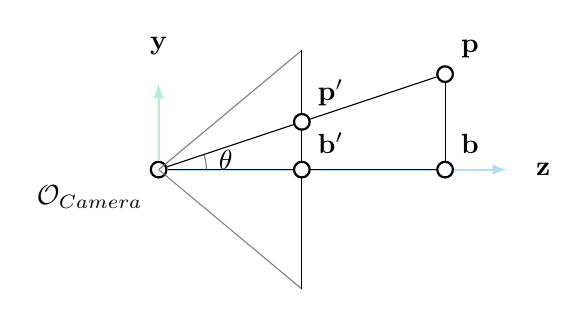
\begin{tikzpicture}
    \node (origin) at (0,0) [coord-point, label=below left:{$\mathcal{O}_{\text{Camera}}$}] {};
    \draw[gray] (0.05\textwidth, 0) arc (0:18.5:0.05\textwidth);

    \node (z-end) at (0.375\textwidth, 0) [label=right:{$\mathbf{z}$}] {};
    \node (y-end) at (0, 0.1\textwidth) [label={$\mathbf{y}$}] {};

    \draw[-latex, tile1, thick] (origin) -- (z-end);
    \draw[-latex, tile2, thick] (origin) -- (y-end);

    \coordinate (theta) at (0.0425\textwidth, 0.01\textwidth);
    \node (theta-node) at (theta) [label=right:{$\theta$}] {};

    \node (p) at (0.3\textwidth, 0.1\textwidth) [coord-point, label=above right:{$\mathbf{p}$}] {};
    \node (p-z) at (0.3\textwidth, 0.\textwidth) [coord-point, label=above right:{$\mathbf{b}$}] {};

    \coordinate (z-near-top) at (0.15\textwidth, 0.125\textwidth) {};
    \coordinate (z-near-bottom) at (0.15\textwidth, -0.125\textwidth) {};

    \draw[-, gray] (origin.center) -- (z-near-top);
    \draw[-, gray] (origin.center) -- (z-near-bottom);
    \draw[-] (z-near-top.center) -- (z-near-bottom);

    \draw[-] (origin) -- (p);
    \draw[-] (origin) -- (p-z);
    \draw[-] (p) -- (p-z);

    \node (p-z-prime) at (0.15\textwidth, 0.\textwidth) [coord-point, label=above right:{$\mathbf{b}^\prime$}] {};
    \node (p-prime) at (0.15\textwidth, 0.05\textwidth) [coord-point, label=above right:{$\mathbf{p}^\prime$}] {};
  \end{tikzpicture}
  \caption{Projectie van een enkel punt.}
  \label{fig:vp-projectie-punt}
\end{figure}
